\chapter{Preliminary Results}
\label{ch:results}

All numbers in this chapter are on the complete HybridQA dev set (\nTest{} questions) unless stated otherwise, and every selector is paired with the same frozen MiniLM reader. Learned selectors are reported as mean and standard deviation over seeds, and their checkpoints were chosen on the validation split. Absolute scores are far below published HybridQA systems (Table~\ref{tab:hybridqa-published}), which fine-tune their readers on HybridQA or use large language models; here the reader is a small SQuAD model that was never trained on tables, and only the selector changes between rows. The comparison is therefore between selection strategies, not between complete question-answering systems.

\section{Headroom for a learned selector}
\label{sec:headroom}

The first question is whether selection matters at all for this reader. Table~\ref{tab:main} answers it. When the reader is given the best traced gold path, an average of \itemsOracle{} entities, it reaches \fOracle{} F1. The best fixed heuristic, BM25 top-3, reaches \fBmThree{} F1 while passing almost twice as many entities, and the greedy rank-then-hop rule used by HYBRIDER-style pipelines reaches \fGreedy{}. A random walk over the same candidate sets scores below 10. The gap of more than 30 points between the heuristics and the oracle is the room a better selector can claim; it is large because the reader is good at extracting answers from the right evidence and poor at ignoring distractors. Dense retrieval, the selection step of TableRAG-style pipelines, is the weakest of the non-random heuristics at every $k$ (\fDenseTwo{} F1 at $k=2$). A likely reason is that the rows of one table are topically almost identical, so embedding similarity separates them poorly, whereas BM25 rewards exact matches of the names and numbers that usually identify the right row.

\begin{table}[t]
\centering
\footnotesize
\caption{Results on the HybridQA dev set (\nTest{} questions) with the same frozen reader for every selector. Learned selectors: mean $\pm$ standard deviation over seeds (number of seeds in brackets). F1$_\mathrm{tab}$, F1$_\mathrm{psg}$: questions whose answer is in a cell (\nTestTypeTable) or a passage (\nTestTypePassage). AnsRec: answer string present in the evidence. Loc: the entity holding a traced answer location is selected. Path: a traced gold path is fully covered (row and passage). Items, Words: evidence passed to the reader.}
\label{tab:main}
\setlength{\tabcolsep}{2.9pt}
\begin{tabular}{@{}lccccccccc@{}}
\toprule
Selector & EM & F1 & F1$_\mathrm{tab}$ & F1$_\mathrm{psg}$ & AnsRec & Loc & Path & Items & Words \\
\midrule
\multicolumn{10}{@{}l}{\textit{No learning}} \\
Random walk, $k{=}2$ [3] & 5.5\,{\scriptsize$\pm$0.1} & 8.6\,{\scriptsize$\pm$0.2} & 14.6 & 4.9 & 12.7 & 12.2 & 7.4 & 2.00 & 136 \\
Random walk, $k{=}3$ [3] & 6.5\,{\scriptsize$\pm$0.3} & 9.6\,{\scriptsize$\pm$0.3} & 15.3 & 6.1 & 17.7 & 17.4 & 10.7 & 3.00 & 214 \\
BM25 top-2 & 13.8 & 18.6 & 21.0 & 17.6 & 29.1 & 27.7 & 10.7 & 2.00 & 219 \\
BM25 top-3 & 15.9 & 20.8 & 21.7 & 21.0 & 37.7 & 36.4 & 18.5 & 3.00 & 333 \\
Dense top-2 (TableRAG) & 10.0 & 13.7 & 19.2 & 10.7 & 21.1 & 20.9 & 12.2 & 2.00 & 151 \\
Dense top-3 & 11.1 & 14.8 & 20.3 & 11.8 & 27.5 & 27.3 & 18.5 & 3.00 & 219 \\
Hybrid top-2 & 13.9 & 18.5 & 22.0 & 16.9 & 28.6 & 27.6 & 12.2 & 2.00 & 199 \\
Hybrid top-3 & 14.9 & 19.8 & 22.1 & 18.9 & 37.6 & 36.5 & 21.0 & 3.00 & 297 \\
Greedy rank-then-hop & 12.9 & 17.4 & 21.2 & 15.7 & 30.5 & 31.4 & 31.4 & 2.00 & 184 \\
\midrule
\multicolumn{10}{@{}l}{\textit{Learned selectors}} \\
Behaviour cloning [5] & 14.1\,{\scriptsize$\pm$0.3} & 19.0\,{\scriptsize$\pm$0.3} & 21.0 & 18.4 & 36.4 & 37.4 & 37.4 & 1.78 & 163 \\
GRPO, warm-started [5] & 11.5\,{\scriptsize$\pm$0.3} & 16.1\,{\scriptsize$\pm$0.5} & 21.9 & 12.9 & 25.8 & 26.2 & 26.2 & 1.33 & 92 \\
PPO + GAE, warm-started [5] & 14.1\,{\scriptsize$\pm$0.3} & 18.9\,{\scriptsize$\pm$0.4} & 21.4 & 18.1 & 35.4 & 36.3 & 36.3 & 1.70 & 152 \\
REINFORCE, warm-started [5] & 15.0\,{\scriptsize$\pm$0.5} & 20.0\,{\scriptsize$\pm$0.5} & 21.5 & 19.9 & 37.2 & 38.3 & 38.2 & 1.82 & 169 \\
\textbf{PPO + GAE from scratch [3]} & \textbf{23.3\,{\scriptsize$\pm$0.2}} & \textbf{28.8\,{\scriptsize$\pm$0.3}} & 35.7 & 25.2 & 50.3 & 49.9 & 33.8 & 2.63 & 331 \\
\midrule
\multicolumn{10}{@{}l}{\textit{Upper bound}} \\
Oracle gold path & 48.4 & 55.7 & 78.6 & 42.9 & 96.9 & 100.0 & 100.0 & 1.58 & 135 \\
\bottomrule
\end{tabular}
\end{table}


\section{Main comparison}

\paragraph{PPO from scratch is the best selector.} PPO trained from a random initialisation reaches \emScratch{} EM and \fScratch{}$\pm$\fScratchStd{} F1, the highest of all non-oracle selectors on every accuracy and evidence-recall metric except full gold-path coverage. Table~\ref{tab:tests} shows that its advantage is far outside the noise: \dScratchBc{} F1 over behaviour cloning (95\% interval [\dScratchBcLo, \dScratchBcHi]), \dScratchBm{} over the best heuristic (BM25 top-3; [\dScratchBmLo, \dScratchBmHi]) and \dScratchGreedy{} over the greedy rank-then-hop rule, with one-sided bootstrap $p$-values below 0.001 and every PPO run better than every run of each comparison method. The gain is not confined to one question type: in-table F1 rises from \ftabBc{} (BC) to \ftabScratch{}, and in-passage F1 from \fpsgBc{} to \fpsgScratch{}.

\paragraph{Warm-started optimisers stay where behaviour cloning put them.} Behaviour cloning on the traced evidence gives \fBc{} F1, roughly level with the hybrid and BM25 heuristics but with fewer entities. PPO started from the cloned policy ends at \fPpo{}, a difference of \dPpoBc{} F1 ([\dPpoBcLo, \dPpoBcHi]), which is no difference at all. REINFORCE from the same start gains a small but significant \dReinforceBc{} F1 ([\dReinforceBcLo, \dReinforceBcHi]). GRPO is worse than its starting point, with a difference of \dGrpoBc{} F1 ([\dGrpoBcLo, \dGrpoBcHi]); Section~\ref{sec:dynamics} explains why.

\begin{table}[t]
\centering
\footnotesize
\caption{Paired comparisons on the dev set. $\Delta$ is the difference A$-$B in points with a 95\% paired-bootstrap interval over questions (10{,}000 resamples, per-question scores averaged over seeds) and the one-sided bootstrap $p$-value for A $\le$ B. $P(\mathrm{A}>\mathrm{B})$: probability that a run of A has a higher F1 than a run of B (deterministic baselines count as one run).}
\label{tab:tests}
\setlength{\tabcolsep}{4pt}
\begin{tabular}{@{}llccccc@{}}
\toprule
A & B & $\Delta$EM [95\% CI] & $p$ & $\Delta$F1 [95\% CI] & $p$ & $P(\mathrm{A}>\mathrm{B})$ \\
\midrule
PPO scratch & BC & +9.23 [+7.94, +10.50] & $<$0.001 & +9.80 [+8.51, +11.09] & $<$0.001 & 1.00 \\
PPO scratch & PPO warm & +9.27 [+7.98, +10.53] & $<$0.001 & +9.84 [+8.54, +11.13] & $<$0.001 & 1.00 \\
PPO scratch & REINFORCE & +8.36 [+7.11, +9.59] & $<$0.001 & +8.74 [+7.47, +10.02] & $<$0.001 & 1.00 \\
PPO scratch & BM25 top-3 & +7.41 [+6.35, +8.49] & $<$0.001 & +7.97 [+6.86, +9.07] & $<$0.001 & 1.00 \\
PPO scratch & Hybrid top-3 & +8.48 [+7.37, +9.58] & $<$0.001 & +9.00 [+7.87, +10.10] & $<$0.001 & 1.00 \\
PPO scratch & Greedy hop & +10.44 [+9.13, +11.76] & $<$0.001 & +11.36 [+10.00, +12.72] & $<$0.001 & 1.00 \\
PPO warm & BC & $-$0.04 [$-$0.31, +0.24] & 0.623 & $-$0.04 [$-$0.31, +0.25] & 0.609 & 0.50 \\
REINFORCE & BC & +0.87 [+0.37, +1.38] & $<$0.001 & +1.06 [+0.55, +1.58] & $<$0.001 & 1.00 \\
GRPO & BC & $-$2.58 [$-$3.10, $-$2.07] & 1.000 & $-$2.90 [$-$3.44, $-$2.37] & 1.000 & 0.00 \\
REINFORCE & PPO warm & +0.91 [+0.43, +1.42] & $<$0.001 & +1.10 [+0.59, +1.61] & $<$0.001 & 1.00 \\
\bottomrule
\end{tabular}
\end{table}


\section{What the learned policy does differently}
\label{sec:behaviour}

Figure~\ref{fig:sizes} and the evidence columns of Table~\ref{tab:main} show that PPO from scratch has learned a different selection strategy rather than a better version of the cloned one. The cloned policy, like its traced targets, always selects exactly one row and adds a passage for 78\% of the questions. PPO from scratch selects three entities for 73\% of the questions, but on average only 0.69 of them are rows. For 35.4\% of the questions it selects no row at all, so all of its evidence comes from the globally best-matching passages; for 60.0\% it selects one row and for the remaining 4.6\% two or more. As a result the answer string is present in its evidence for \ansrecScratch\% of the questions, against \ansrecBc\% for behaviour cloning and \ansrecBmThree\% for BM25 top-3, and the entity holding a traced answer location is selected for \locScratch\% of the questions, against \locBc\%.

Two checks guard against reading too much into this. Full gold-path coverage, which requires both the row and the passage of a traced path, is lower for PPO from scratch (\pathScratch\%) than for behaviour cloning (\pathBc\%), simply because the policy often skips the row; the answer-location metric shows that it still finds the answer-bearing entity more often. And right answers obtained without selecting any traced answer location are rare for every selector: the highest rate, for PPO from scratch, is 0.53\% of the questions. The improvement therefore does not come from accidental string matches elsewhere in the evidence.

\begin{figure}[t]
\centering
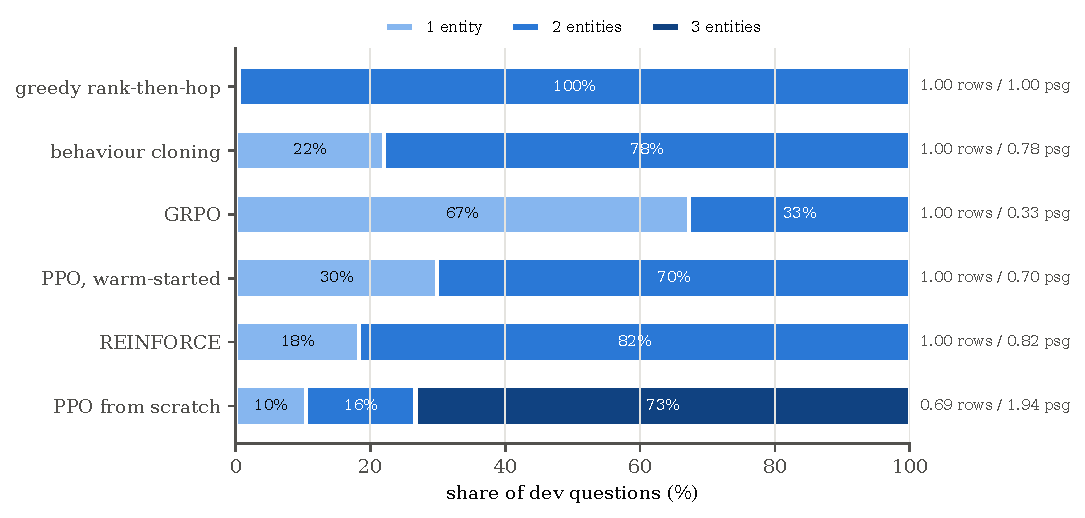
\includegraphics[width=0.92\textwidth]{figures/sizes.pdf}
\caption{Number of entities each selector passes to the reader on the dev set (learned selectors pooled over seeds), with the average numbers of rows and passages on the right.}
\label{fig:sizes}
\end{figure}

Selecting more entities is not, by itself, what makes the difference. Figure~\ref{fig:tradeoff} places every selector by the amount of text it passes to the reader. PPO from scratch uses about as many words as BM25 top-3 (\wordsScratch{} against \wordsBmThree{}), but scores \dScratchBm{} F1 more; taking more entities from any heuristic ranking helps much less. Within the warm-started family the entity cost has little room to act: for $c$ between 0 and 0.1 the evidence length stays between 151 and 169 words, with no monotone trend beyond $c=0$, and F1 varies by less than one point.

\begin{figure}[t]
\centering
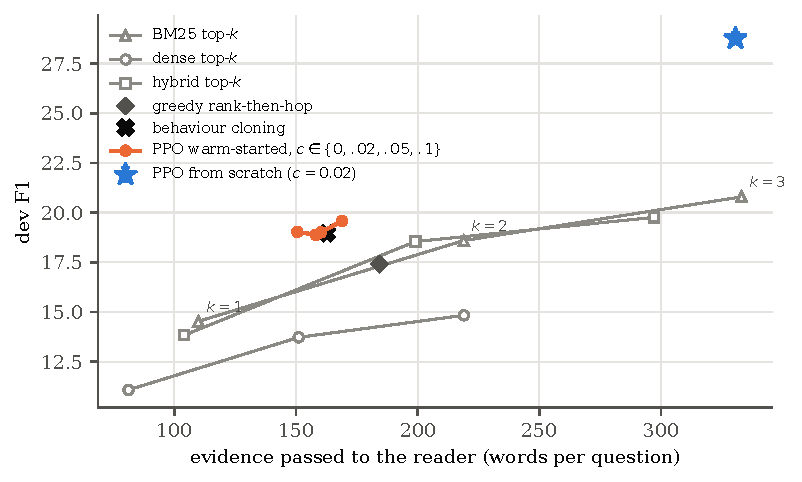
\includegraphics[width=0.85\textwidth]{figures/tradeoff.pdf}
\caption{Dev F1 against the evidence passed to the reader. Grey: top-$k$ heuristics for $k=1,2,3$. Orange: warm-started PPO with entity cost $c\in\{0,0.02,0.05,0.1\}$ (seeds 0--2). Blue star: PPO from scratch (three seeds; bar: standard deviation).}
\label{fig:tradeoff}
\end{figure}

\section{Learning dynamics}
\label{sec:dynamics}

Figure~\ref{fig:curves} shows validation F1 during training and Figure~\ref{fig:diagnostics} the training diagnostics; Table~\ref{tab:optim} summarises them.

\begin{figure}[t]
\centering
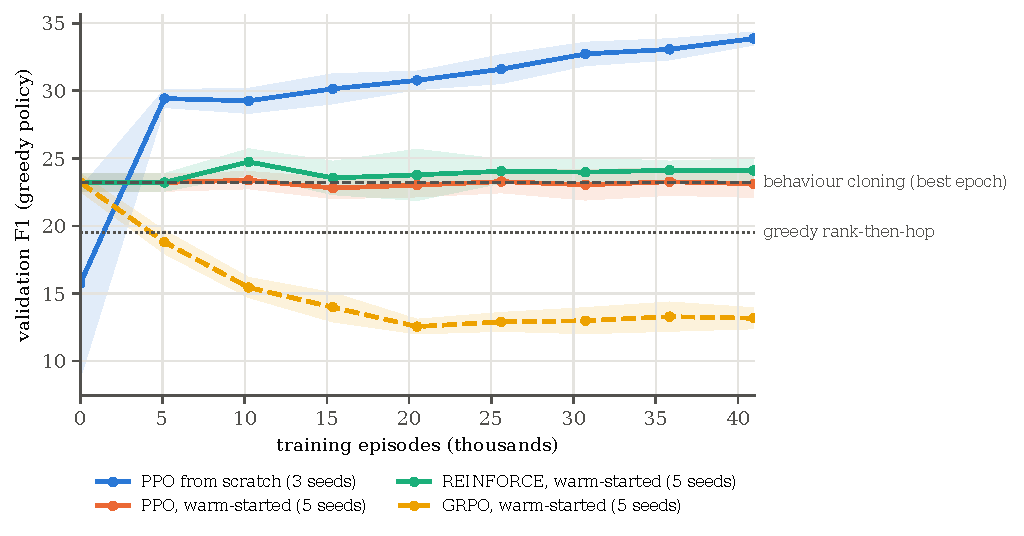
\includegraphics[width=0.9\textwidth]{figures/curves.pdf}
\caption{Validation F1 of the greedy policy during training (mean over seeds; band: $\pm$ one standard deviation). Every method sees 1{,}024 episodes per iteration. Episode~0 is the starting policy: the cloned policy for the warm-started methods, a random network for PPO from scratch.}
\label{fig:curves}
\end{figure}

\paragraph{PPO from scratch.} The randomly initialised policy starts at \initScratch{} validation F1, passes every other selector within the first five iterations, and is still improving when training stops (best validation F1 \valScratch{}, reached at the last iteration for all three seeds). Its sampled training F1 and its greedy validation F1 stay close (0.36 and 0.34 at the end), and its critic reaches an explained variance of about \evScratch{}. Over training the policy uses slightly fewer entities (from 2.86 to \itemsEndScratch{} per episode) and ends more episodes with an explicit \STOP{} (from 9\% to 22\%), which is the per-entity cost at work.

\paragraph{Warm-started PPO and REINFORCE.} Both start from the cloned policy at \initPpo{} validation F1. PPO's mean curve stays within one point of it, and REINFORCE gains one to two points. Their critics learn well (explained variance \evPpo{} and \evReinforce{}), and their sampled training F1 rises from 0.22 to 0.28--0.29, but the greedy validation score hardly follows. The policy updates are small: PPO's mean approximate KL per update is 0.003 and only 3\% of ratios are clipped, against 0.006 and 8\% for PPO from scratch, and the policy entropy falls from 0.80 to 0.40 nats. In words, the warm-started policies become more certain of the choices behaviour cloning taught them, and the improvement on training questions does not transfer. Behaviour cloning itself overfits: averaged over the five seeds, its training accuracy on oracle steps rises from 0.51 to 0.82 over eight epochs, while its validation loss is lowest after the third epoch and rises afterwards.

\paragraph{GRPO.} GRPO's validation F1 falls from \initGrpo{} to about 13 within twenty iterations, and the number of entities per episode collapses from 1.7 to \itemsEndGrpo. On average \degenGrpo\% of its groups receive identical returns and therefore no gradient. We think the collapse comes from the remaining groups. When the four answers of a group are equally wrong, the returns differ only through the per-entity cost, and dividing by the small within-group standard deviation turns differences of 0.02 into advantages of order one, which teaches the policy to stop as early as possible. We did not log per-group answer scores, so this explanation is an inference from the collapse in entity counts, not a measurement. It is the failure mode \citet{liu2025understanding} attribute to standard-deviation normalisation, and it matches the advantage collapse reported by \citet{wang2026igpo}.

\paragraph{Checkpoint selection.} The validation evaluation at iteration 5 happens before any actor update of the warm-started methods, because their critic-only warm-up lasts five iterations. For the iterate chosen at iteration 5, the reported model is therefore the cloned policy itself. This happened for PPO seed~0 among the main runs and for one or two seeds of several ablations (the ``Best it.'' column of Table~\ref{tab:ablation}); in all of these cases no later PPO iterate scored higher on validation, so the choice reflects the flat learning curves rather than changing the conclusions.

\begin{figure}[t]
\centering
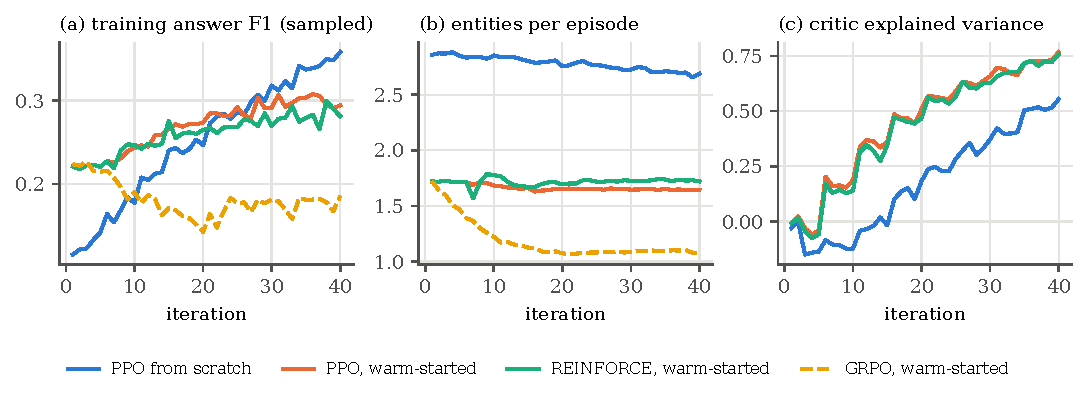
\includegraphics[width=\textwidth]{figures/diagnostics.pdf}
\caption{Training diagnostics per iteration, averaged over seeds: (a) F1 of the sampled episodes on training questions, (b) entities selected per episode, (c) explained variance of the critic (PPO and REINFORCE).}
\label{fig:diagnostics}
\end{figure}

\begin{table}[t]
\centering
\footnotesize
\caption{Training behaviour of the optimisers (same data, reward, evaluation and per-iteration episode budget). Init: initial validation F1 of the starting policy. Best val: validation F1 of the selected iterate (iteration in brackets, mean over seeds). EV: explained variance of the critic on the last batch. Items: entities per training episode at the last iteration. Time: minutes of training iterations per run (periodic validation excluded) on one T4 GPU.}
\label{tab:optim}
\setlength{\tabcolsep}{4pt}
\begin{tabular}{@{}lcccccc@{}}
\toprule
Method & Init & Best val (iter.) & Dev F1 & EV (end) & Items (end) & Time \\
\midrule
PPO + GAE from scratch & 15.8 & 33.9 (40) & 28.8\,{\scriptsize$\pm$0.3} & 0.55 & 2.69 & 2.2 \\
PPO + GAE, warm-started from BC & 23.2 & 23.7 (17) & 18.9\,{\scriptsize$\pm$0.4} & 0.77 & 1.64 & 1.7 \\
REINFORCE + baseline, warm-started & 23.2 & 25.1 (21) & 20.0\,{\scriptsize$\pm$0.5} & 0.76 & 1.72 & 1.2 \\
GRPO, warm-started & 23.2 & 18.8 (5) & 16.1\,{\scriptsize$\pm$0.5} & n/a & 1.08 & 0.9 \\
\bottomrule
\end{tabular}
\end{table}


\section{Reward and advantage ablations}
\label{sec:ablations}

Table~\ref{tab:ablation} varies the evidence term, the answer metric, the GAE parameter and the entity cost of the warm-started PPO configuration. All rows lie within 0.8 F1 of each other, which is about twice the seed standard deviation, and no setting moves the policy far from the cloned one. The largest values come from the settings that give the policy the most freedom or the noisiest signal, $c=0$ (19.6 F1) and $\lambda=1$ (19.5), but these differences are not significant at three seeds. The comparison between potential-based shaping and a terminal evidence bonus (G4) is therefore inconclusive in the warm-started regime: neither form changed what PPO learned, which is what the theory predicts for shaping but not necessarily for the bonus. The informative version of this experiment is to repeat it from scratch, where the policy does move (Chapter~\ref{ch:conclusion}).

\begin{table}[t]
\centering
\footnotesize
\caption{Ablations of the warm-started PPO configuration on the dev set (seeds 0--2 for every row, including the main configuration). Best it.: validation-selected iteration per seed. Path: a traced gold path is covered. R/L: exact match although no traced answer location is selected.}
\label{tab:ablation}
\setlength{\tabcolsep}{4pt}
\begin{tabular}{@{}llcccccc@{}}
\toprule
Factor & Setting & EM & F1 & Path & R/L & Items & Best it. \\
\midrule
Reward form & no evidence term & 14.1\,{\scriptsize$\pm$0.2} & 19.2\,{\scriptsize$\pm$0.1} & 36.7 & 0.1 & 1.73 & 5, 15, 25 \\
 & shaping, $\kappa=0.5$ (main) & 14.1\,{\scriptsize$\pm$0.4} & 19.0\,{\scriptsize$\pm$0.4} & 36.8 & 0.1 & 1.75 & 5, 10, 30 \\
 & terminal bonus, $\lambda_{\mathrm{ev}}=0.3$ & 14.2\,{\scriptsize$\pm$0.0} & 19.2\,{\scriptsize$\pm$0.1} & 37.4 & 0.1 & 1.75 & 15, 40, 20 \\
 & shaping, EM instead of F1 & 14.0\,{\scriptsize$\pm$0.3} & 19.0\,{\scriptsize$\pm$0.4} & 37.2 & 0.1 & 1.77 & 5, 20, 10 \\
\midrule
GAE $\lambda$ & $\lambda=0$ & 13.8\,{\scriptsize$\pm$0.4} & 18.8\,{\scriptsize$\pm$0.5} & 36.1 & 0.1 & 1.71 & 5, 35, 15 \\
 & $\lambda=0.95$ (main) & 14.1\,{\scriptsize$\pm$0.4} & 19.0\,{\scriptsize$\pm$0.4} & 36.8 & 0.1 & 1.75 & 5, 10, 30 \\
 & $\lambda=1$ & 14.5\,{\scriptsize$\pm$0.1} & 19.5\,{\scriptsize$\pm$0.2} & 37.9 & 0.1 & 1.77 & 10, 20, 20 \\
\midrule
Entity cost $c$ & $c=0$ & 14.5\,{\scriptsize$\pm$0.3} & 19.6\,{\scriptsize$\pm$0.4} & 38.3 & 0.1 & 1.81 & 10, 20, 25 \\
 & $c=0.02$ (main) & 14.1\,{\scriptsize$\pm$0.4} & 19.0\,{\scriptsize$\pm$0.4} & 36.8 & 0.1 & 1.75 & 5, 10, 30 \\
 & $c=0.05$ & 14.1\,{\scriptsize$\pm$0.3} & 19.0\,{\scriptsize$\pm$0.4} & 36.5 & 0.1 & 1.69 & 15, 10, 20 \\
 & $c=0.1$ & 14.0\,{\scriptsize$\pm$0.5} & 18.9\,{\scriptsize$\pm$0.6} & 36.4 & 0.1 & 1.74 & 5, 10, 5 \\
\bottomrule
\end{tabular}
\end{table}


\section{Generalisation checks}
\label{sec:unseen}

\paragraph{Unseen tables.} Because HybridQA's splits share tables, \testQuestionsWithTrainTable{} dev questions use a table that also occurs in our training subset. Table~\ref{tab:unseen} splits the dev set accordingly. On the questions whose table is unseen, PPO from scratch reaches \fScratchUnseen{} F1, against \fBcUnseen{} for behaviour cloning and \fBmThreeUnseen{} for BM25 top-3, so the gain does not depend on having seen the table.

\begin{table}[t]
\centering
\footnotesize
\caption{Dev results split by whether the question's table occurs in the training subset.}
\label{tab:unseen}
\begin{tabular}{@{}lcccc@{}}
\toprule
 & \multicolumn{2}{c}{Unseen tables (3,163 questions)} & \multicolumn{2}{c}{Seen tables (303 questions)} \\
\cmidrule(lr){2-3}\cmidrule(l){4-5}
Selector & EM & F1 & EM & F1 \\
\midrule
BM25 top-3 & 15.9 & 20.6 & 16.5 & 22.3 \\
Hybrid top-3 & 14.7 & 19.4 & 16.8 & 23.3 \\
Greedy rank-then-hop (HYBRIDER-style) & 12.8 & 17.4 & 13.9 & 17.7 \\
Behaviour cloning (BC) & 14.0\,{\scriptsize$\pm$0.3} & 18.8\,{\scriptsize$\pm$0.3} & 15.4\,{\scriptsize$\pm$0.5} & 20.7\,{\scriptsize$\pm$0.2} \\
GRPO, warm-started & 11.5\,{\scriptsize$\pm$0.3} & 15.9\,{\scriptsize$\pm$0.4} & 12.4\,{\scriptsize$\pm$0.8} & 17.5\,{\scriptsize$\pm$0.8} \\
PPO + GAE, warm-started from BC & 14.0\,{\scriptsize$\pm$0.4} & 18.8\,{\scriptsize$\pm$0.5} & 15.0\,{\scriptsize$\pm$0.8} & 20.4\,{\scriptsize$\pm$0.9} \\
REINFORCE + baseline, warm-started & 14.9\,{\scriptsize$\pm$0.5} & 19.9\,{\scriptsize$\pm$0.5} & 15.8\,{\scriptsize$\pm$1.0} & 21.3\,{\scriptsize$\pm$0.8} \\
PPO + GAE from scratch & 23.3\,{\scriptsize$\pm$0.2} & 28.6\,{\scriptsize$\pm$0.2} & 23.3\,{\scriptsize$\pm$1.0} & 30.7\,{\scriptsize$\pm$1.4} \\
Oracle gold path & 48.6 & 55.8 & 46.2 & 54.0 \\
\bottomrule
\end{tabular}
\end{table}


\paragraph{A second reader.} Table~\ref{tab:reader} keeps every selector's evidence fixed and replaces the reader by RoBERTa-base, which was never used in training, on the first 1{,}000 dev questions. The ranking of the selectors does not change. PPO from scratch reaches \robScratch{} F1 with the new reader, against \robBmThree{} for BM25 top-3, \robReinforce{} for REINFORCE and \robBc{} for behaviour cloning, while the oracle reaches \robOracle{}; most selectors gain a little from the stronger reader, and PPO from scratch gains slightly more than the others (from \miniScratch{} to \robScratch{} on these questions). The learned selection is therefore not tied to the quirks of the reader it was trained with. So that the table is internally consistent, all of its second-reader entries were computed in one environment (the laptop CPU) from the stored selections; as a check, re-reading behaviour cloning's seed-0 selections there gave 16.0 EM / 20.4 F1, against 15.8 / 20.2 in the GPU environment.

\begin{table}[t]
\centering
\footnotesize
\caption{Transfer to a second frozen reader (RoBERTa-base SQuAD~2.0) that was never used during training, on the first 1{,}000 dev questions (the dev file is ordered by a hashed question id). Each selector's evidence is exactly what it selected in the main evaluation; only the reader changes. The oracle is recomputed under the new reader. Left: the training reader's scores on the same questions.}
\label{tab:reader}
\begin{tabular}{@{}lcccc@{}}
\toprule
 & \multicolumn{2}{c}{Training reader (MiniLM)} & \multicolumn{2}{c}{Unseen reader (RoBERTa)} \\
\cmidrule(lr){2-3}\cmidrule(l){4-5}
Selector & EM & F1 & EM & F1 \\
\midrule
Dense top-2 (TableRAG-style) & 10.4 & 14.1 & 11.1 & 14.3 \\
Hybrid top-2 & 14.9 & 19.5 & 16.1 & 20.2 \\
Hybrid top-3 & 14.9 & 19.8 & 16.0 & 20.8 \\
BM25 top-3 & 15.9 & 20.5 & 16.5 & 21.1 \\
Greedy rank-then-hop (HYBRIDER-style) & 13.6 & 18.4 & 14.0 & 18.0 \\
Behaviour cloning (BC) & 13.8\,{\scriptsize$\pm$0.6} & 19.1\,{\scriptsize$\pm$0.5} & 16.0\,{\scriptsize$\pm$0.5} & 20.5\,{\scriptsize$\pm$0.3} \\
GRPO, warm-started & 10.9\,{\scriptsize$\pm$0.8} & 15.7\,{\scriptsize$\pm$0.9} & 12.0\,{\scriptsize$\pm$0.8} & 16.2\,{\scriptsize$\pm$1.0} \\
PPO + GAE, warm-started from BC & 13.5\,{\scriptsize$\pm$0.6} & 18.9\,{\scriptsize$\pm$0.7} & 15.3\,{\scriptsize$\pm$0.8} & 20.0\,{\scriptsize$\pm$0.8} \\
REINFORCE + baseline, warm-started & 15.0\,{\scriptsize$\pm$0.7} & 20.5\,{\scriptsize$\pm$0.7} & 16.3\,{\scriptsize$\pm$0.8} & 21.1\,{\scriptsize$\pm$0.8} \\
PPO + GAE from scratch & 23.7\,{\scriptsize$\pm$0.1} & 28.7\,{\scriptsize$\pm$0.0} & 25.5\,{\scriptsize$\pm$0.3} & 30.8\,{\scriptsize$\pm$0.5} \\
Oracle gold path & 49.0 & 56.7 & 54.2 & 61.4 \\
\bottomrule
\end{tabular}
\end{table}



\section{Compute}
\label{sec:compute}

Preparing the data (graph construction and embedding of 230{,}512 entity texts) took 5.2 hours on the laptop CPU, most of it under battery throttling. On the laptop, one reader call costs about 120~ms, so a single PPO run with the reader in the loop would take several hours. All reported training and evaluation therefore ran on one NVIDIA T4 GPU, where the complete suite (baselines, 5 behaviour-cloning runs, 42 reinforcement-learning runs, all dev evaluations and the second-reader experiment) took 1.17 hours. A PPO run of 40 iterations takes 1--3 minutes there (Table~\ref{tab:optim}), most of it Python-side environment stepping; the policy itself is too small to matter. The decomposable reader and its cache are what make this possible: every (question, entity) pair is read once and reused by all methods, seeds and iterations.
